% ===================================================================
%  Week 11 — Session 1: Transforms & the Homography Model
% ===================================================================
\documentclass[10pt,aspectratio=169]{beamer}
% ===================================================================
%  Shared Beamer preamble for "Practical Image Processing"
%  English slides. Compile with pdfLaTeX.
% ===================================================================

\usetheme{metropolis}
\usepackage[T1]{fontenc}
\usepackage[utf8]{inputenc}
\usepackage{lmodern}
\usepackage{listings}
\usepackage{tcolorbox}
\usepackage{fontawesome5}
\usepackage{booktabs}
\usepackage{amsmath,amssymb}
\usepackage{tikz}
\usepackage{pgfplots}
\pgfplotsset{compat=1.17}
\usetikzlibrary{arrows.meta,positioning,shapes.geometric,fit,backgrounds,matrix}
\tcbuselibrary{skins,breakable}

% ---- Palette --------------------------------------------------------
\definecolor{coursePrimary}{HTML}{1B4965}   % deep blue
\definecolor{courseAccent}{HTML}{E76F51}    % coral
\definecolor{courseGood}{HTML}{2A9D8F}      % teal
\definecolor{courseBad}{HTML}{C0392B}       % red
\definecolor{courseInfo}{HTML}{2980B9}      % blue
\definecolor{codeBg}{HTML}{F5F6FA}
\definecolor{codeKw}{HTML}{8E44AD}
\definecolor{codeStr}{HTML}{2A9D8F}
\definecolor{codeCom}{HTML}{7F8C8D}

\setbeamercolor{frametitle}{bg=coursePrimary}
\setbeamercolor{progress bar}{fg=courseAccent}
\setbeamercolor{alerted text}{fg=courseAccent}
\metroset{block=fill,sectionpage=progressbar,numbering=fraction}

% ---- Code listings (Python is built into listings) -----------------
\lstdefinestyle{course}{
  backgroundcolor=\color{codeBg},
  basicstyle=\ttfamily\scriptsize,
  keywordstyle=\color{codeKw}\bfseries,
  stringstyle=\color{codeStr},
  commentstyle=\color{codeCom}\itshape,
  numberstyle=\tiny\color{codeCom},
  numbers=left, numbersep=6pt,
  showstringspaces=false, breaklines=true, breakatwhitespace=true,
  tabsize=4, columns=fullflexible,
  frame=single, framesep=4pt, rulecolor=\color{gray!30},
  keepspaces=true, upquote=true, language=Python,
}
\lstset{style=course}
\lstdefinelanguage{bash}{
  keywords={cd,pip,python,venv,source,import}, sensitive=true,
  morecomment=[l]{\#}, morestring=[b]', morestring=[b]",
}

% ---- Reusable callout boxes ----------------------------------------
\newtcolorbox{goodbox}[1][Good practice]{colback=courseGood!8,colframe=courseGood,
  fonttitle=\bfseries,title={\faCheck~#1},boxrule=0.6pt,left=4pt,right=4pt,top=3pt,bottom=3pt}
\newtcolorbox{badbox}[1][Pitfall]{colback=courseBad!8,colframe=courseBad,
  fonttitle=\bfseries,title={\faTimes~#1},boxrule=0.6pt,left=4pt,right=4pt,top=3pt,bottom=3pt}
\newtcolorbox{infobox}[1][Note]{colback=courseInfo!8,colframe=courseInfo,
  fonttitle=\bfseries,title={\faInfoCircle~#1},boxrule=0.6pt,left=4pt,right=4pt,top=3pt,bottom=3pt}
\newtcolorbox{mathbox}[1][Math]{colback=coursePrimary!6,colframe=coursePrimary,
  fonttitle=\bfseries,title={\faCalculator~#1},boxrule=0.6pt,left=4pt,right=4pt,top=3pt,bottom=3pt}

\newcommand{\keyidea}[1]{\begin{alertblock}{Key idea}#1\end{alertblock}}
\newcommand{\term}[1]{\textbf{\color{coursePrimary}#1}}
\newcommand{\code}[1]{\lstinline[basicstyle=\ttfamily\small]|#1|}

% ---- A helper to draw a small pixel grid, cells shaded by value ----
% \pixelgrid{ {10,20,120,200,240}, {30,60,130,180,230}, ... }
\newcommand{\pixelgrid}[1]{%
  \begin{tikzpicture}[font=\scriptsize,scale=0.6]
    \foreach \row [count=\ry] in {#1} {
      \foreach \val [count=\cx] in \row {
        \draw[gray,fill=coursePrimary!8] (\cx,-\ry) rectangle ++(1,-1);
        \node at (\cx+0.5,-\ry-0.5) {\val};
      }
    }
  \end{tikzpicture}}


\title{Homography \& Perspective Warp}
\subtitle{Week 11 — Session 1: Transforms \& the Homography Model}
\author{Practical Image Processing}
\date{Lecture 11.1 \textbullet\ 60--70 min}

\begin{document}

\maketitle

\begin{frame}{Where we are}
  \begin{columns}[T]
    \begin{column}{0.58\textwidth}
      \begin{itemize}
        \item Wk10: we matched the same points across two views of a scene.
        \item \alert{This session:} the \emph{maths of moving pixels} — the family of
              2D transforms, and the one that models a camera: the \term{homography}.
        \item Next session we \emph{use} it: warp an angled photo of a meter/document
              into a flat, front-on scan.
      \end{itemize}
    \end{column}
    \begin{column}{0.42\textwidth}
      \begin{alertblock}{Two-session arc}
        \textbf{S1 (today):} the models — affine, projective, homogeneous coords.\\[3pt]
        \textbf{S2:} the pipeline — rectify, interpolate, RANSAC, DocScan.
      \end{alertblock}
    \end{column}
  \end{columns}
\end{frame}

\begin{frame}{Roadmap}\tableofcontents\end{frame}

% ==================================================================
\section{Positions, not values}
% ==================================================================

\begin{frame}{What is a geometric transform?}
  \begin{itemize}
    \item So far we changed pixel \emph{values} (brightness, edges). Now we change pixel \emph{positions}.
    \item A geometric transform maps each output pixel $(x',y')$ back to a source location $(x,y)$.
    \item Examples: translate, rotate, scale, shear, and — the big one — \term{perspective}.
  \end{itemize}
  \keyidea{Value operations answer ``what colour is here?'' Geometric operations answer ``where does this point go?''}
\end{frame}

\begin{frame}{Forward vs.\ inverse mapping}
  \begin{columns}[T]
    \begin{column}{0.54\textwidth}
      \begin{itemize}
        \item \term{Forward}: push each source pixel to its destination. Leaves holes and overlaps.
        \item \term{Inverse}: for each \emph{output} pixel, ask where it came from in the source, then sample.
        \item Real warpers use inverse mapping — every output pixel gets exactly one value.
      \end{itemize}
    \end{column}
    \begin{column}{0.46\textwidth}
      \begin{center}
      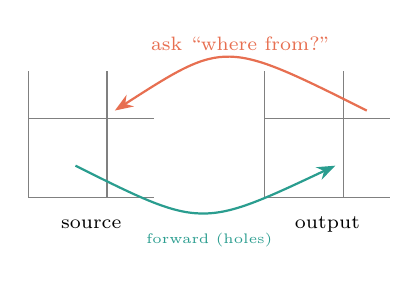
\begin{tikzpicture}[font=\scriptsize,>=Stealth]
        \draw[gray] (0,0) grid (1.6,1.6);
        \node at (0.8,-0.35) {source};
        \draw[gray] (3.0,0) grid (4.6,1.6);
        \node at (3.8,-0.35) {output};
        \draw[->,courseAccent,thick] (4.3,1.1) .. controls (2.5,2.0) .. (1.1,1.1);
        \node[courseAccent] at (2.7,1.95) {ask ``where from?''};
        \draw[->,courseGood,thick] (0.6,0.4) .. controls (2.2,-0.4) .. (3.9,0.4);
        \node[courseGood] at (2.3,-0.55) {\tiny forward (holes)};
      \end{tikzpicture}
      \end{center}
    \end{column}
  \end{columns}
  \begin{infobox}
    Inverse mapping is why \code{cv2.warpPerspective} takes the transform \emph{output$\to$input} internally.
  \end{infobox}
\end{frame}

% ==================================================================
\section{The transform hierarchy}
% ==================================================================

\begin{frame}{A hierarchy of 2D transforms}
  \begin{center}
  \begin{tabular}{@{}llll@{}}
    \toprule
    \textbf{Transform} & \textbf{Preserves} & \textbf{DoF} & \textbf{Matrix} \\
    \midrule
    Rigid (rotate+translate) & lengths, angles & 3 & $2\times3$ \\
    Similarity (+scale) & angles, ratios & 4 & $2\times3$ \\
    Affine & parallelism & 6 & $2\times3$ \\
    Projective (homography) & straight lines only & 8 & $3\times3$ \\
    \bottomrule
  \end{tabular}
  \end{center}
  \keyidea{Each row is more general. A photo taken at an angle needs the most general one: a \term{homography}.}
\end{frame}

\begin{frame}{The hierarchy, visually}
  \begin{center}
  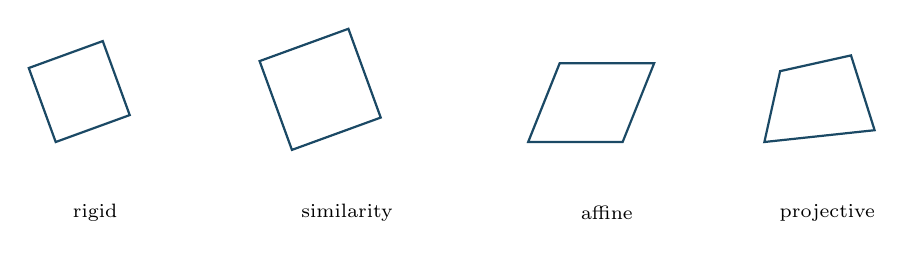
\begin{tikzpicture}[font=\scriptsize,node distance=6mm]
    \tikzset{sq/.style={draw,coursePrimary,thick}}
    % rigid: rotated square
    \begin{scope}[shift={(0,0)},rotate=20]
      \draw[sq] (0,0) rectangle (1,1);
    \end{scope}
    \node at (0.5,-0.9) {rigid};
    % similarity: bigger rotated square
    \begin{scope}[shift={(3,-0.1)},rotate=20,scale=1.2]
      \draw[sq] (0,0) rectangle (1,1);
    \end{scope}
    \node at (3.7,-0.9) {similarity};
    % affine: parallelogram
    \begin{scope}[shift={(6,0)}]
      \draw[sq] (0,0) -- (1.2,0) -- (1.6,1) -- (0.4,1) -- cycle;
    \end{scope}
    \node at (1.0+6,-0.9) {affine};
    % projective: general quad
    \begin{scope}[shift={(9,0)}]
      \draw[sq] (0,0) -- (1.4,0.15) -- (1.1,1.1) -- (0.2,0.9) -- cycle;
    \end{scope}
    \node at (0.8+9,-0.9) {projective};
  \end{tikzpicture}
  \end{center}
  \vspace{2pt}
  Left to right: fewer things kept fixed. The unit square becomes a rotated square, a scaled one,
  a parallelogram, and finally an arbitrary (but still straight-edged) quadrilateral.
\end{frame}

\begin{frame}{Rigid \& similarity in matrix form}
  \begin{mathbox}
    Rotation by $\theta$ then translation $t$:
    \[
      \begin{pmatrix}x'\\y'\end{pmatrix}=
      \underbrace{\begin{pmatrix}\cos\theta & -\sin\theta\\ \sin\theta & \cos\theta\end{pmatrix}}_{R}
      \begin{pmatrix}x\\y\end{pmatrix}+\begin{pmatrix}t_x\\t_y\end{pmatrix}
    \]
    Similarity multiplies $R$ by a scalar scale $s$ (4 DoF: $\theta, s, t_x, t_y$).
  \end{mathbox}
  \begin{itemize}
    \item $R$ is orthonormal: columns are unit length and perpendicular $\Rightarrow$ no stretching or shear.
    \item That is exactly why rigid motion keeps lengths and angles.
  \end{itemize}
\end{frame}

\begin{frame}{Affine transform}
  \begin{itemize}
    \item 6 degrees of freedom: a $2\times3$ matrix. Maps parallelograms to parallelograms.
    \item \code{cv2.getAffineTransform(3 pts, 3 pts)}, then \code{cv2.warpAffine}.
    \item Good for rotation/scale/shear — but \emph{cannot} model a page tilted away from the camera.
  \end{itemize}
  \begin{mathbox}
    Affine: $\begin{pmatrix}x'\\y'\end{pmatrix} = A\begin{pmatrix}x\\y\end{pmatrix} + t$,
    with $A=\begin{pmatrix}a&b\\c&d\end{pmatrix}$. Straight, parallel lines stay parallel.
  \end{mathbox}
\end{frame}

\begin{frame}{Worked example: a shear + scale}
  \begin{columns}[T]
    \begin{column}{0.55\textwidth}
      \begin{mathbox}
        $A=\begin{pmatrix}1 & 0.5\\ 0 & 1\end{pmatrix}$, $t=\begin{pmatrix}0\\0\end{pmatrix}$
      \end{mathbox}
      Map the unit square's corners:
      \begin{itemize}
        \item $(0,0)\!\to\!(0,0)$
        \item $(1,0)\!\to\!(1,0)$
        \item $(0,1)\!\to\!(0.5,1)$
        \item $(1,1)\!\to\!(1.5,1)$
      \end{itemize}
      Bottom edge fixed, top edge slid right by $0.5\,y$: a horizontal shear.
    \end{column}
    \begin{column}{0.45\textwidth}
      \begin{center}
      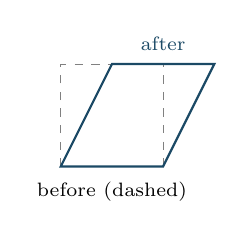
\begin{tikzpicture}[font=\scriptsize,scale=1.3]
        \draw[gray,dashed] (0,0) rectangle (1,1);
        \draw[coursePrimary,thick] (0,0)--(1,0)--(1.5,1)--(0.5,1)--cycle;
        \node at (0.5,-0.25) {before (dashed)};
        \node[coursePrimary] at (1.0,1.2) {after};
      \end{tikzpicture}
      \end{center}
    \end{column}
  \end{columns}
\end{frame}

\begin{frame}{Affine vs perspective — on a grid}
  \begin{columns}[T]
    \begin{column}{0.5\textwidth}\begin{center}
      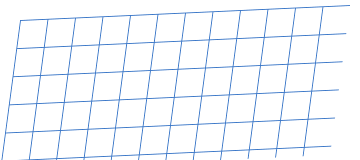
\includegraphics[width=0.95\linewidth]{../assets/grid_affine.png}\\{\scriptsize affine: parallel lines stay parallel}
    \end{center}\end{column}
    \begin{column}{0.5\textwidth}\begin{center}
      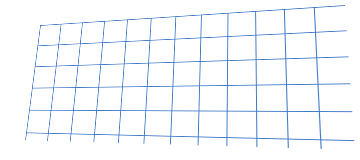
\includegraphics[width=0.95\linewidth]{../assets/grid_perspective.png}\\{\scriptsize perspective: parallel lines converge}
    \end{center}\end{column}
  \end{columns}
  \vspace{3pt}
  The converging lines are the ``vanishing point'' effect of a real camera. Only a homography models it.
\end{frame}

% ==================================================================
\section{Homogeneous coordinates}
% ==================================================================

\begin{frame}{Why homogeneous coordinates?}
  \begin{itemize}
    \item Affine needs a matrix \emph{plus} an added vector $t$ — clumsy to chain.
    \item Trick: append a 1. A point $(x,y)$ becomes $(x,y,1)$; now translation is a \emph{matrix multiply}.
    \item Bonus: it lets us express \term{points at infinity} $(x,y,0)$ — the vanishing points.
  \end{itemize}
  \begin{mathbox}
    Affine as one $3\times3$ multiply:
    $\begin{pmatrix}x'\\y'\\1\end{pmatrix}=
     \begin{pmatrix}a&b&t_x\\ c&d&t_y\\ 0&0&1\end{pmatrix}
     \begin{pmatrix}x\\y\\1\end{pmatrix}$
  \end{mathbox}
\end{frame}

\begin{frame}{Points at infinity \& vanishing points}
  \begin{itemize}
    \item Set $w=0$: $(x,y,0)$ is a \term{point at infinity} — a pure \emph{direction}, not a location.
    \item Two parallel lines share the same direction, so they meet at the same point at infinity.
    \item A homography can send $w=0$ to a finite $w'\neq0$: infinity lands \emph{on-image} as a \term{vanishing point}.
  \end{itemize}
  \keyidea{``Parallel rails meeting at the horizon'' is literally a point at infinity mapped to a finite pixel.}
\end{frame}

\begin{frame}{Chaining transforms is matrix multiplication}
  \begin{itemize}
    \item Homogeneous form makes composition trivial: do $H_1$ then $H_2$ $=$ apply $H_2H_1$ (right-to-left).
    \item Undo a transform with its inverse $H^{-1}$; warpers use it for inverse mapping.
    \item So ``rotate about a point $c$'' $=$ translate by $-c$, rotate, translate back: $T_{c}RT_{-c}$.
  \end{itemize}
  \begin{mathbox}
    $H_{\text{about }c}=T(c)\,R(\theta)\,T(-c)$ — three simple $3\times3$ matrices multiplied into one.
  \end{mathbox}
  \begin{goodbox}
    Precompute the product once; then a single multiply warps every pixel.
  \end{goodbox}
\end{frame}

\begin{frame}{Scale invariance: $(x,y,w)\equiv(\lambda x,\lambda y,\lambda w)$}
  \begin{itemize}
    \item A homogeneous point is defined only \emph{up to a nonzero scale}: $(2,4,2)$ and $(1,2,1)$ are the same point.
    \item To read off the pixel, \term{normalise}: divide by the last coordinate $\to (x/w,\,y/w)$.
    \item This single ``divide'' is where perspective will hide (next section).
  \end{itemize}
  \begin{goodbox}
    Always normalise before plotting: a returned $(x',y',w')$ with $w'\neq1$ is not yet a pixel.
  \end{goodbox}
\end{frame}

% ==================================================================
\section{The homography}
% ==================================================================

\begin{frame}{The homography}
  \begin{itemize}
    \item A \term{homography} $H$ is a $3\times3$ matrix relating two views of a \emph{planar} surface.
    \item 8 degrees of freedom (the 9th is a scale). Maps straight lines to straight lines, but
          parallel lines may converge.
    \item Exactly the model for photographing a flat page/meter from any angle.
  \end{itemize}
  \begin{mathbox}
    $\begin{pmatrix}x'\\y'\\w'\end{pmatrix} = H\begin{pmatrix}x\\y\\1\end{pmatrix}$,
    $\quad H=\begin{pmatrix}h_{11}&h_{12}&h_{13}\\ h_{21}&h_{22}&h_{23}\\ h_{31}&h_{32}&1\end{pmatrix}$,
    then divide by $w'$.
  \end{mathbox}
\end{frame}

\begin{frame}{Why divide by $w'$? (the perspective part)}
  \begin{itemize}
    \item That final division is what makes far things smaller and parallel lines converge.
    \item Affine has bottom row $(0\ 0\ 1)$ $\Rightarrow$ $w'=1$ always $\Rightarrow$ no perspective.
    \item Homography's bottom row $(h_{31}\ h_{32}\ 1)$ makes $w'$ depend on position $\Rightarrow$ perspective.
  \end{itemize}
  \keyidea{The nonlinear ``divide by $w'$'' is the whole difference between affine and perspective.}
\end{frame}

\begin{frame}{Worked example: one point through $H$}
  \begin{columns}[T]
    \begin{column}{0.52\textwidth}
      \begin{mathbox}
        $H=\begin{pmatrix}1&0&0\\0&1&0\\0.001&0&1\end{pmatrix}$
      \end{mathbox}
      Push $(x,y)=(400,300)$:
      \begin{align*}
        w' &= 0.001(400)+1 = 1.4\\
        x' &= 400,\quad y'=300\\
        \text{pixel} &= (400/1.4,\,300/1.4)\\
                     &\approx (286,\,214)
      \end{align*}
    \end{column}
    \begin{column}{0.48\textwidth}
      \begin{itemize}
        \item Only $h_{31}=0.001$ is nonzero, yet the point moved inward.
        \item Points with larger $x$ get a larger $w'$, so they shrink more $\Rightarrow$ a wall recedes.
        \item Set $h_{31}=h_{32}=0$ and it collapses back to a pure affine map.
      \end{itemize}
    \end{column}
  \end{columns}
\end{frame}

\begin{frame}{How many points define a homography?}
  \begin{itemize}
    \item 8 unknowns $\Rightarrow$ need 8 equations $\Rightarrow$ \term{4 point correspondences} (each gives 2).
    \item \code{cv2.getPerspectiveTransform(4 src, 4 dst)} for exactly 4 points.
    \item With many noisy matches: \code{cv2.findHomography(pts, pts, cv2.RANSAC)} (next session).
  \end{itemize}
  \begin{goodbox}
    4 good corners is all you need. For DocScan, those 4 are the document's corners.
  \end{goodbox}
\end{frame}

\begin{frame}{Setting up the equations (a peek at the DLT)}
  \begin{itemize}
    \item Each correspondence $(x,y)\!\to\!(x',y')$ expands the ratios and clears the denominator $w'$.
    \item That yields \emph{two} linear equations in the 8 unknowns per point.
  \end{itemize}
  \begin{mathbox}
    From $x'=\dfrac{h_{11}x+h_{12}y+h_{13}}{h_{31}x+h_{32}y+1}$, multiply up:
    \[ h_{11}x+h_{12}y+h_{13}-x'(h_{31}x+h_{32}y)=x' \]
    Four points $\Rightarrow$ 8 such rows $\Rightarrow$ solve $A\mathbf{h}=\mathbf{b}$ (or SVD for the noisy case).
  \end{mathbox}
  \begin{infobox}
    OpenCV does all of this inside \code{getPerspectiveTransform}; the point is to know it is just linear algebra.
  \end{infobox}
\end{frame}

% ==================================================================
\section{In-class exercise}
% ==================================================================

\begin{frame}{\faPen~In-class exercise (10 min)}
  \begin{infobox}[Reason about the models]
  \end{infobox}
  \begin{enumerate}
    \item Which is the simplest transform that can rotate \emph{and} uniformly enlarge a logo? How many DoF?
    \item Write the homogeneous $3\times3$ matrix for a pure translation of $(+30,-10)$.
    \item A homography returns $(x',y',w')=(600,900,3)$. What pixel is that?
    \item Why can an affine transform never make two parallel rails meet at the horizon?
  \end{enumerate}
\end{frame}

\begin{frame}{\faPen~Debrief}
  \begin{itemize}
    \item (1) A \term{similarity} (rotation + uniform scale + translation): 4 DoF.
    \item (2) $\begin{pmatrix}1&0&30\\0&1&-10\\0&0&1\end{pmatrix}$.
    \item (3) Normalise: $(600/3,\,900/3)=(200,\,300)$.
    \item (4) Its bottom row is $(0\ 0\ 1)$, so $w'\equiv1$: no per-point division, hence no convergence.
  \end{itemize}
  \keyidea{Everything reduces to: build a matrix, multiply, divide by $w'$. The model choice sets what stays fixed.}
\end{frame}

% ==================================================================
\section{Pitfalls \& good practice}
% ==================================================================

\begin{frame}{Common pitfalls with the models}
  \begin{badbox}[Using affine where you need projective]
    A page tilted away from the camera has converging edges. \code{warpAffine} will straighten
    rotation but leave a keystone — the far edge stays too small.
  \end{badbox}
  \begin{badbox}[Forgetting to normalise]
    Plotting $(x',y')$ without dividing by $w'$ puts points wildly off-image. Always divide.
  \end{badbox}
\end{frame}

\begin{frame}{Good practice}
  \begin{goodbox}[Pick the least powerful model that fits]
    More DoF = more freedom to overfit noise. Use rigid/affine when the scene really is fronto-parallel;
    reserve the homography for genuine perspective.
  \end{goodbox}
  \begin{goodbox}[Keep everything in homogeneous form]
    Chaining transforms is just matrix products $H_2H_1$. Convert to pixels only at the very end.
  \end{goodbox}
\end{frame}

% ==================================================================
\section{Wrap-up}
% ==================================================================

\begin{frame}{What you should now be able to do}
  \begin{itemize}
    \item Place a transform in the hierarchy (rigid $\to$ similarity $\to$ affine $\to$ projective) and count its DoF.
    \item Write rigid, affine, and projective maps in homogeneous $3\times3$ form.
    \item Explain \emph{why} the divide-by-$w'$ step is the entire source of perspective.
    \item Argue why 4 correspondences (8 equations) pin down a homography.
  \end{itemize}
\end{frame}

\begin{frame}{Next session}
  \begin{alertblock}{S2 — from model to scanner}
    We turn the homography into the \term{DocScan} pipeline:
    \begin{itemize}
      \item order the 4 corners and pick a destination rectangle,
      \item \code{warpPerspective} with the right \term{interpolation},
      \item and align \emph{automatically} from feature matches using \term{RANSAC}.
    \end{itemize}
  \end{alertblock}
  Come with today's mental model: build $H$, multiply, divide by $w'$.
\end{frame}

\begin{frame}[standout]
  A transform is just a matrix and a division.\\[4pt]
  \normalsize Choose what stays fixed; the homography fixes only straight lines — enough to model a camera.
\end{frame}

\end{document}
